% Appendix for Major Project Report (2026-27)

\begin{appendices}

\chapter{Project Planning}

\section{Project Timeline}
The project was planned as a 30-week schedule from 15 February 2026 to 16 October 2026. The work was divided into the phases listed in Table~\ref{tab:timeline}: literature and requirements, environment and data preparation, graph construction and baselines, GNN design and training, export and inference service, SDN integration, mitigation, dashboard and testing, and the final documentation. Work was shared among the four team members; the allocation of each workstream is given in Table~\ref{tab:alloc}.

\subsection{Project Timeline}

The project timeline illustrates the planned phases of project development, including requirement analysis, literature survey, design, implementation, testing, validation, and documentation.

\begin{longtable}{|p{1.0cm}|p{3.4cm}|p{3.0cm}|p{7.2cm}|}
\caption{Project timeline (30 weeks)}\label{tab:timeline}\\
\hline
\textbf{Week} & \textbf{Phase} & \textbf{Dates} & \textbf{Main activities and outputs} \\ \hline
\endfirsthead
\hline \textbf{Week} & \textbf{Phase} & \textbf{Dates} & \textbf{Main activities and outputs} \\ \hline
\endhead
1--2 & Requirement analysis and literature survey & 15 Feb -- 28 Feb 2026 & Literature on SDN security, GNNs and IDS datasets; InSDN and CICIDS2017 structure; problem statement, objectives, success metrics; OpenFlow 1.3, Mininet and os-ken study; feature mapping. \\ \hline
3--4 & Environment and data survey & 1 Mar -- 14 Mar 2026 & Virtual environment, repository structure, Docker image with Mininet, OVS and os-ken; InSDN download and inspection; feature-schema draft. \\ \hline
5--6 & Data cleaning and labels & 15 Mar -- 28 Mar 2026 & \texttt{clean\_data.py} (deduplication, types, missing values); label mapping and class-imbalance strategy. \\ \hline
7--8 & Graph construction and EDA & 29 Mar -- 11 Apr 2026 & Window aggregation, host graphs, serialisation; validation of node/edge counts and features; EDA and graph visualisation. \\ \hline
9--10 & Baselines & 12 Apr -- 25 Apr 2026 & Random Forest and XGBoost; common splits; evaluation, per-class analysis and Phase~1 write-up. \\ \hline
11--13 & GNN design and first training & 26 Apr -- 16 May 2026 & Shared GAT encoder, graph head and node head, loss weighting; PyTorch Geometric implementation; training loop and unit tests; first experiments and debugging. \\ \hline
14--16 & Tuning, ablation and comparison & 17 May -- 6 Jun 2026 & Hyper-parameter search; ablations (features, tasks, depth); fair comparison table RF vs XGBoost vs GNN; results in \texttt{results/phase2/}. \\ \hline
17--18 & Export and inference service & 7 Jun -- 20 Jun 2026 & TorchScript export and check, latency benchmark; inference engine, alert classifier, FastAPI service. \\ \hline
19 & Controller & 21 Jun -- 27 Jun 2026 & os-ken app, 2~s flow-stats polling, forwarding to the IDS. \\ \hline
20--21 & Mininet laboratory and integration & 1 Aug -- 14 Aug 2026 & Topology with attackers, victim and benign hosts; Docker lab; benign and attack traffic scripts; controller $\to$ IDS $\to$ dashboard data flow. \\ \hline
22--24 & Mitigation & 15 Aug -- 11 Sep 2026 & Policy per attack type, rule expiry, whitelist; drop, meter and isolation actions; audit log; live pipeline tests. \\ \hline
25--26 & Dashboard & 5 Sep -- 18 Sep 2026 & Offline results page; live monitor with traffic graph, alerts, rules and manual block/unblock. \\ \hline
27--28 & Testing and stress tests & 19 Sep -- 2 Oct 2026 & Pytest suite for preprocessing, model, inference, controller, mitigation; sustained-attack tests; latency and false-positive tuning. \\ \hline
29--30 & Final results and documentation & 3 Oct -- 16 Oct 2026 & Final results, README, Docs and execution guide; demo script and rehearsal; project report and presentation. \\ \hline
\end{longtable}

\begin{table}[htbp]
\centering
\caption{Allocation of workstreams among team members}
\label{tab:alloc}
\small
\begin{tabularx}{\textwidth}{|p{5.5cm}|X|}
\hline
\textbf{Workstream} & \textbf{Team member(s)} \\ \hline
Data cleaning, labels, graph construction, EDA & \textit{(to be filled in by the team)} \\ \hline
Baselines, GNN training, ablations, feature selection & \textit{(to be filled in by the team)} \\ \hline
Inference service, export, latency benchmarks & \textit{(to be filled in by the team)} \\ \hline
Controller, Mininet laboratory, attack scripts & \textit{(to be filled in by the team)} \\ \hline
Mitigation engine, dashboard, tests & \textit{(to be filled in by the team)} \\ \hline
Report, poster, paper and presentation & \textit{(to be filled in by the team)} \\ \hline
\end{tabularx}
\end{table}

\section{Budget Estimation}
The project is entirely software based. It uses open-source software, a public dataset and an emulated network, so no hardware had to be bought. Table~\ref{tab:budget} lists the resources and the estimated cost; the figures marked ``estimate'' are indicative.

\begin{table}[htbp]
\centering
\caption{Resources and estimated budget}
\label{tab:budget}
\small
\begin{tabularx}{\textwidth}{|c|p{5.2cm}|X|r|}
\hline
\textbf{Sl. No.} & \textbf{Resource} & \textbf{Remarks} & \textbf{Cost (INR)} \\ \hline
1 & Development and training machine (laptop with NVIDIA RTX 3050 GPU, 8 GB or more memory) & Already owned by the team; the CPU alone is sufficient for inference & 0 (existing) \\ \hline
2 & Python, PyTorch, PyTorch Geometric, scikit-learn, XGBoost, FastAPI & Open source & 0 \\ \hline
3 & Mininet, Open vSwitch, os-ken, hping3, nmap, iperf3, tcpdump, Docker & Open source & 0 \\ \hline
4 & InSDN dataset & Publicly available for research & 0 \\ \hline
5 & GitHub repository & Free plan & 0 \\ \hline
6 & Internet and electricity during development & Estimate & 2,000 \\ \hline
7 & Printing and binding of the report, poster & Estimate & 1,500 \\ \hline
\multicolumn{3}{|r|}{\textbf{Total estimated additional expenditure}} & \textbf{3,500} \\ \hline
\end{tabularx}
\end{table}

A hardware deployment would additionally need an OpenFlow-capable switch (or a Raspberry Pi/PC with Open vSwitch), several hosts and a server for the IDS service; this was out of scope because Mininet reproduces the required OpenFlow behaviour.


\section{Risk Analysis}
\begin{table}[htbp]
\centering
\caption{Project risks and the actions taken}
\label{tab:risks}
\small
\begin{tabularx}{\textwidth}{|p{4.0cm}|c|X|}
\hline
\textbf{Risk} & \textbf{Impact} & \textbf{Mitigation / what happened} \\ \hline
Dataset has no IP addresses (CICIDS2017 variant) & High & Switched to InSDN for the host graphs; documented in the design decisions. \\ \hline
Controller (Ryu) does not install on current Python & Medium & Used the os-ken fork with a launcher script. \\ \hline
Mininet needs root and a supported distribution & Medium & Privileged Docker image with host networking; IDS kept on the host. \\ \hline
Inflated offline results from window overlap & High & Time-ordered split with a gap and a unit test. \\ \hline
Model does not transfer to the lab & High & Collected labelled laboratory runs and fine-tuned; checked that InSDN performance is preserved. \\ \hline
Benign hosts blocked by automatic mitigation & High & Mean host score, two-window persistence, whitelist, priorities, expiry. \\ \hline
Slow first inference calls & Medium & Warm-up at start (p99 208~ms $\to$ 11~ms). \\ \hline
Gap in the schedule (weeks 19 to 20) & Low & The plan has no activity between 27 June and 1 August; the remaining weeks were scheduled consecutively afterwards. \\ \hline
\end{tabularx}
\end{table}

\chapter{Sustainable Development Goals (SDGs) Addressed}
The project contributes mostly to goals concerning digital infrastructure and security, and in a smaller way to education, economic growth and sustainable communities. Table~\ref{tab:sdg-impact} shows the rating of each goal on the scale defined below the table; only the goals with a meaningful contribution are discussed.

\begin{table}[htbp]
	\centering
	\caption{SDG Impact Evaluation}
	\label{tab:sdg-impact}
	\begin{tabular}{|p{10cm}|c|}
		\hline
		\textbf{Sustainable Development Goal} & \textbf{Level} \\
		\hline
		No Poverty & 1 \\ \hline
		Zero Hunger & 1 \\ \hline
		Good Health and Well-being & 1 \\ \hline
		Quality Education & 2 \\ \hline
		Gender Equality & 1 \\ \hline
		Clean Water and Sanitation & 1 \\ \hline
		Affordable and Clean Energy & 1 \\ \hline
		Decent Work and Economic Growth & 2 \\ \hline
		Industry, Innovation and Infrastructure & 3 \\ \hline
		Reduced Inequalities & 1 \\ \hline
		Sustainable Cities and Communities & 2 \\ \hline
		Responsible Consumption and Production & 1 \\ \hline
		Climate Action & 1 \\ \hline
		Life Below Water & 1 \\ \hline
		Life on Land & 1 \\ \hline
		Peace, Justice and Strong Institutions & 3 \\ \hline
		Partnerships for the Goals & 2 \\ \hline
	\end{tabular}
\end{table}

\noindent\textbf{Levels:} Poor = 1, Good = 2, Excellent = 3.

\subsection{SDGs with the Highest Contribution}

The project shows an excellent contribution (level 3) to SDG 9 and SDG 16, and a good contribution (level 2) to SDG 4, SDG 8, SDG 11 and SDG 17.

\textbf{SDG 9: Industry, Innovation and Infrastructure (level 3):}
Networks are the infrastructure on which all digital services run. The project provides a method for protecting SDN infrastructure that detects attacks, identifies the attacking hosts and mitigates them automatically within seconds, and does this with features an ordinary OpenFlow switch reports, so that it can be applied to existing equipment. Combining graph neural networks with software-defined networking is also an innovation in network operations.

\textbf{SDG 16: Peace, Justice and Strong Institutions (level 3):}
Denial-of-service and scanning attacks disrupt institutions, and manual response is slow. Automatic detection with an audit log of every action, a whitelist for critical infrastructure and expiring rules supports secure, accountable and reliable digital institutions.

\textbf{SDG 11: Sustainable Cities and Communities (level 2):}
Smart-city services and public networks depend on available and secure networks. Faster protection against floods keeps connected services running.

\textbf{SDG 4: Quality Education (level 2) and SDG 8: Decent Work and Economic Growth (level 2):}
The reproducible pipeline, the documentation and the Docker laboratory can be reused for teaching network security and machine learning, and the skills used (SDN, GNNs, MLOps) are in demand in the industry. Automatic response reduces the cost of outages for businesses.

\textbf{SDG 17: Partnerships for the Goals (level 2):}
The project is based on open-source tools and a public dataset, its source code is available in a public repository, and every result file records the configuration and code version, so that others can reproduce and extend it. It combines networking, cybersecurity, machine learning and software engineering.

\chapter{Self-Assessment of the Project}
The project was evaluated against the Program Outcomes (POs) and Program Specific Outcomes (PSOs) to assess the extent to which the engineering knowledge, technical skills, problem-solving abilities, professional practices, and project management capabilities were demonstrated during the project development process. The assessment reflects the contribution of the project towards achieving the defined graduate attributes and program-specific competencies. The contribution levels are categorized as Poor (1), Good (2), and Excellent (3).

\section{Self-Assessment of the Project}

\begin{longtable}{|c|p{5.2cm}|p{7cm}|c|}
	\caption{Self-Assessment of the Project Outcomes}
	\label{tab:self-assessment}\\
	\hline
	\textbf{No.} & \textbf{PO and PSO} & \textbf{Contribution from the Project} & \textbf{Level} \\
	\hline
	\endfirsthead

	\hline
	\textbf{No.} & \textbf{PO and PSO} & \textbf{Contribution from the Project} & \textbf{Level} \\
	\hline
	\endhead

	1 &
	Engineering Knowledge &
	Applied graph theory, probability and information theory (entropy), machine learning, deep learning on graphs, computer networks (TCP/IP, OpenFlow) and cybersecurity to design the IDS. &
	3 \\ \hline

	2 &
	Problem Analysis &
	Analysed the limits of flow-level IDS and of offline-only evaluation, found dataset problems (no IP addresses in CICIDS2017 files, flow-direction noise, split leakage) and formulated a graph-based, OpenFlow-compatible solution. &
	3 \\ \hline

	3 &
	Design and Development of Solutions &
	Designed the feature schema, graph builder, multi-task GAT, inference service, controller integration and the mitigation policy with safety rails. &
	3 \\ \hline

	4 &
	Conduct Investigations of Complex Problems &
	Ran baselines, ablations, feature-selection comparison, latency benchmarks, replay tests and 12 live attack runs; used window, host and mitigation metrics and corrected the design on the evidence. &
	3 \\ \hline

	5 &
	Modern Tool Usage &
	Used PyTorch Geometric, TorchScript, scikit-learn, XGBoost, FastAPI, Mininet, Open vSwitch, os-ken, Docker, hping3 and nmap, with the choice of each tool justified. &
	3 \\ \hline

	6 &
	The Engineer and the World &
	Considered the impact of false blocks on legitimate users, fail-open behaviour, rule expiry and the limits of the solution (spoofed DDoS). The system uses no special hardware and low computing power. &
	2 \\ \hline

	7 &
	Ethics &
	Used a public dataset for research, tested attacks only inside an isolated emulated network, reported negative and partial results honestly (rare classes, unmet reaction-time target) and kept an audit log of automatic actions. &
	3 \\ \hline

	8 &
	Individual and Team Work &
	Four members worked on data, model, controller and dashboard components and integrated them through shared configuration and tests. &
	3 \\ \hline

	9 &
	Communication &
	Documented the architecture, feature schema, label scheme, design decisions and execution guide; prepared the report, dashboards and presentation material. &
	3 \\ \hline

	10 &
	Project Management and Finance &
	Followed a 30-week plan with milestones, tracked tasks and used only free and already available resources (Appendix~A). &
	3 \\ \hline

	11 &
	Life-long Learning &
	Learned GNNs, OpenFlow, Mininet, os-ken, TorchScript and meter-based rate limiting beyond the curriculum. &
	3 \\ \hline

	12 &
	PSO1 -- Computer-Based Systems Development &
	Built a complete system of data pipeline, model service, controller, switches and dashboard, running on Linux with containers. &
	3 \\ \hline

	13 &
	PSO2 -- Software Development &
	Developed about 7,400 lines of modular Python with configuration files, REST APIs, logging, 45 automated tests and a web interface. &
	3 \\ \hline

	14 &
	PSO3 -- Computer Communications and Internet Applications &
	Applied OpenFlow, TCP/UDP/ICMP traffic behaviour, flow tables, meters and controller--switch communication to detect and stop network attacks. &
	3 \\ \hline

\end{longtable}

\noindent\textbf{Levels:} Poor = 1, Good = 2, Excellent = 3.


\section{Ethical and Safety Considerations}
Attack tools (hping3, nmap) were used only inside the emulated network of the laboratory, whose hosts are virtual and isolated from other networks. The dataset is public and contains no personal data. The mitigation engine is limited by design: rules expire, whitelisted hosts cannot be blocked, and every action is auditable. The code is intended for defence and teaching, and it does not contain tools for attacking real networks beyond the standard utilities used for traffic generation.

\chapter{Input Details}
\section{Dataset / Input Details}
The primary dataset is \textbf{InSDN} \cite{bib:insdn}, recorded on an SDN testbed (Open vSwitch with a controller, Kali Linux attackers and Metasploitable and web-server victims). It consists of three groups of CSV files with CICFlowMeter flow statistics: \texttt{Normal\_data}, \texttt{OVS} (attacks against the Open vSwitch network) and \texttt{metasploitable-2}. After cleaning (deduplication, type conversion, handling of missing and infinite values) the files contain 343,888 flows (Table~\ref{tab:dataset}). The \texttt{MachineLearningCVE} version of CICIDS2017 \cite{bib:cicids} was used in Phase~1 only; it has no IP addresses, ports or timestamps and is therefore unsuitable for building host graphs.

\begin{table}[htbp]
\centering
\caption{Flows per file and class after cleaning}
\label{tab:dataset}
\small
\begin{tabular}{|l|l|r|r|r|}
\hline
\textbf{File} & \textbf{Class} & \textbf{Flows} & \textbf{Source IPs} & \textbf{Destination IPs} \\ \hline
Normal\_data & Benign & 68,423 & 922 & 1,075 \\ \hline
OVS & Botnet & 164 & 3 & 3 \\ \hline
OVS & BruteForce & 1,110 & 2 & 2 \\ \hline
OVS & DDoS & 48,413 & 48,413 & 3 \\ \hline
OVS & DoS & 52,471 & 2 & 2 \\ \hline
OVS & Probe & 36,372 & 3 & 6 \\ \hline
OVS & WebAttack & 192 & 4 & 3 \\ \hline
metasploitable-2 & BruteForce & 295 & 2 & 3 \\ \hline
metasploitable-2 & DDoS & 73,529 & 73,529 & 1 \\ \hline
metasploitable-2 & DoS & 1,145 & 2 & 2 \\ \hline
metasploitable-2 & Other (U2R) & 17 & 2 & 3 \\ \hline
metasploitable-2 & Probe & 61,757 & 2 & 2 \\ \hline
\end{tabular}
\end{table}

The main observations from the exploratory analysis are: benign and attack traffic come from separate captures; DDoS flows use spoofed sources (one flow per source address); WebAttack, Botnet and Other are very small; timestamps are mostly minute-resolution, so windows are counted in flows; and the flow direction is noisy (Chapter~4). Figures~\ref{fig:structure} and~\ref{fig:examples} show the graph structure of the classes.

\begin{figure}[htbp]
\centering
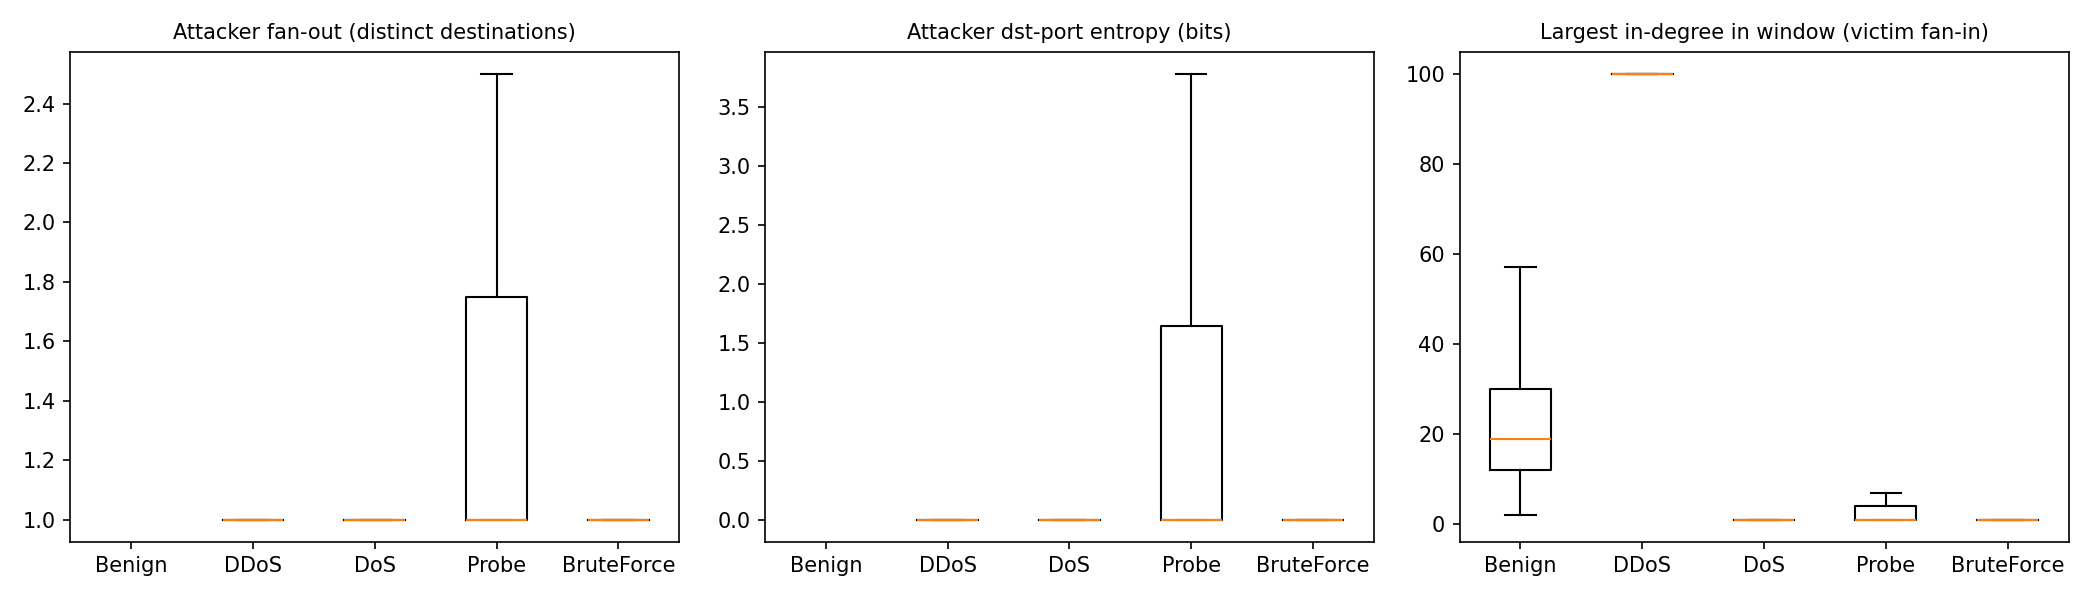
\includegraphics[width=0.9\textwidth]{structure_by_class}
\caption{Graph structure (hosts, attackers, in-degree) by class}
\label{fig:structure}
\end{figure}

\begin{figure}[htbp]
\centering
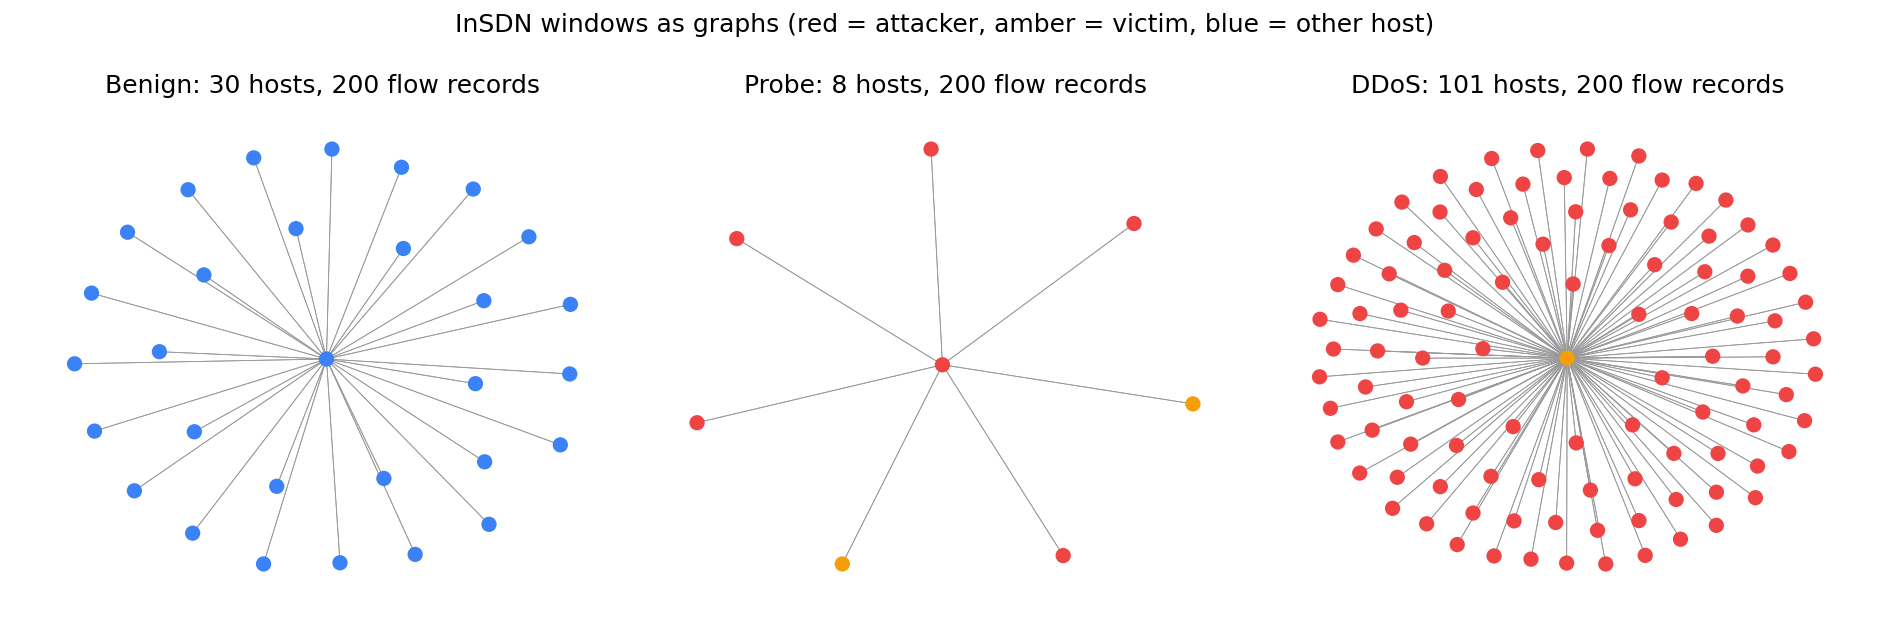
\includegraphics[width=0.9\textwidth]{example_graphs}
\caption{Example window graphs of the classes}
\label{fig:examples}
\end{figure}

\section{Data Collection / Capture Methodology}
\textbf{Offline data.} The InSDN CSV files were used as published. \textbf{Laboratory data} were generated in the Mininet topology (2 Open vSwitch switches, 6 hosts) controlled by the os-ken application. The script \texttt{inject\_attack.py} runs benign background traffic (web clients polling the web server with curl, an iperf3 stream and a ping stream) and, in each run, one scenario: benign, DDoS (hping3 SYN flood with random spoofed sources from both attacker hosts), DoS (hping3 SYN flood from one host), Probe (repeated nmap SYN scans of ports 1--2000) or BruteForce (repeated curl login requests with random passwords to a service port). It records the ground truth of each run (attack type, attacker IPs, victim, start and end times, spoofed or not) as JSON and captures the packets at the victim with tcpdump. With mitigation disabled (\texttt{COLLECT=1}) the IDS records the flows that the controller reports into \texttt{flows.csv}; \texttt{label\_mininet\_flows.py} labels a flow as an attack if, during the attack interval, it goes from an attacker IP (or from any non-topology IP for spoofed DDoS) to the victim, together with the victim's replies, and converts them into graph windows. Runs are split as a whole: the 4th run of each scenario is used for testing and the 5th for validation. Each run lasts 25~s of benign traffic, 45~s of attack and 40~s of benign traffic.

\section{Input Features and Label Encoding}
The 16 edge features and 16 node features are listed in Tables~\ref{tab:edgefeat} and~\ref{tab:nodefeat}. Features are transformed with $\operatorname{sign}(x)\log(1+|x|)$ and standardised with training-split statistics (Eq.~\ref{eq:norm}). The attack classes are encoded as in Table~\ref{tab:labels}; unknown labels map to Other and never to Benign.

\begin{table}[htbp]
\centering
\caption{Label encoding}
\label{tab:labels}
\small
\begin{tabularx}{\textwidth}{|c|l|X|X|}
\hline
\textbf{ID} & \textbf{Class} & \textbf{CICIDS2017 labels} & \textbf{InSDN labels} \\ \hline
0 & Benign & BENIGN & Normal \\ \hline
1 & DDoS & DDoS & DDoS \\ \hline
2 & DoS & DoS Hulk, GoldenEye, slowloris, Slowhttptest, Heartbleed & DoS \\ \hline
3 & Probe & PortScan & Probe \\ \hline
4 & BruteForce & FTP-Patator, SSH-Patator, Web Attack -- Brute Force & BFA \\ \hline
5 & WebAttack & Web Attack -- XSS, SQL Injection & Web-Attack \\ \hline
6 & Botnet & Bot & BOTNET \\ \hline
7 & Other & Infiltration & U2R \\ \hline
\end{tabularx}
\end{table}

\textbf{Window label:} the most frequent attack class if at least 10\% of the initiator-direction records are attacks, otherwise Benign. \textbf{Host label:} 1 if the host initiated at least one attack flow, else 0. \textbf{Binary label:} class $\ne$ Benign.

\chapter{Configuration Details}
\section{System Requirements}
\begin{table}[htbp]
\centering
\caption{Hardware requirements}
\label{tab:hw}
\small
\begin{tabularx}{\textwidth}{|l|X|X|}
\hline
 & \textbf{Minimum (inference and laboratory)} & \textbf{Recommended (training, ablations)} \\ \hline
Processor & 4-core x86-64 CPU & 8-core CPU \\ \hline
Memory & 8 GB & 16 GB \\ \hline
GPU & Not required (the service path is 6.5~ms on CPU) & CUDA GPU (reference machine: NVIDIA RTX 3050 Laptop GPU) \\ \hline
Storage & 10 GB (datasets, graphs, container image) & 20 GB \\ \hline
Network & Loopback (IDS, controller and Mininet on one machine) & Gigabit Ethernet if the IDS runs on a separate host \\ \hline
\end{tabularx}
\end{table}

\section{Software Configuration}
\begin{table}[htbp]
\centering
\caption{Software configuration}
\label{tab:sw}
\small
\begin{tabularx}{\textwidth}{|p{4.2cm}|X|}
\hline
\textbf{Component} & \textbf{Version / details} \\ \hline
Operating system (host) & Arch Linux, kernel 6.19 \\ \hline
Laboratory container & Ubuntu 22.04 with Mininet 2.3, Open vSwitch 2.17, os-ken 2.8.1, hping3, nmap, iperf3, tcpdump (privileged, host networking) \\ \hline
Language & Python 3.14.3 \\ \hline
Machine learning & PyTorch 2.11.0, PyTorch Geometric 2.7.0, scikit-learn 1.8.0, XGBoost 3.2.0 \\ \hline
Data and graphs & pandas 3.0.2, NumPy 2.4.4, NetworkX 3.6.1 \\ \hline
Visualisation & Matplotlib 3.10.9, Seaborn 0.13.2 \\ \hline
Service and dashboard & FastAPI, Uvicorn, HTML/CSS/JavaScript front end \\ \hline
Testing & pytest 9.1.1 (45 tests) \\ \hline
Other & PyYAML 6.0.3, requests 2.33.1, tqdm 4.67.3, Docker, Git \\ \hline
\end{tabularx}
\end{table}

\section{Model and System Configuration}
\begin{table}[htbp]
\centering
\caption{Model, training and live-system parameters}
\label{tab:cfg}
\small
\begin{tabularx}{\textwidth}{|p{4.6cm}|X|}
\hline
\textbf{Parameter} & \textbf{Value} \\ \hline
Graph window (offline) & 100 flows, stride 25 (10 for the benign file), minimum attack fraction 0.1, benign overlay probability 0.5 \\ \hline
Split & 70\% / 15\% / 15\% in time order per (file, class), with a gap; seed 42 \\ \hline
Model & Multi-task GAT: hidden size 64, 4 heads, 2 layers, dropout 0.2, bidirectional message passing, edge features; about 65\,k parameters \\ \hline
Loss and optimiser & $0.5\,\mathcal{L}_{\text{node}}+0.5\,\mathcal{L}_{\text{graph}}$; square-root inverse-frequency class weights (cap 10); AdamW, learning rate $10^{-3}$, weight decay $10^{-4}$, gradient clipping 2.0, learning rate halved after 5 epochs without improvement \\ \hline
Training schedule & Batch 64 graphs, up to 60 epochs, early stopping patience 10 \\ \hline
Baselines & Random Forest (200 trees), XGBoost (300 trees) \\ \hline
Feature selection & Methods: ANOVA, mutual information, RF importance, L1, RFE, PCA, SVD, FastICA; $k\in\{4,6,8,10,12\}$; tolerance 0.005 \\ \hline
Export & TorchScript bundle \texttt{models/gat\_ids.pt} with normalisation statistics, class names, thresholds, feature names \\ \hline
Live window and polling & 10~s window, 2~s polling, chunks of 200 records \\ \hline
Decision thresholds & ATTACK $\ge 0.85$, SUSPICIOUS $\ge 0.5$, node threshold from validation, confirmation in 2 windows, cool-down 30~s, host score = mean over chunks \\ \hline
Mitigation & Rule idle timeout 60~s, hard timeout 300~s, victim rate limit 200 packets/s (hard timeout 120~s), scanner rate limit 20 packets/s, spoof threshold 20 sources, heavy-hitter threshold 5 flows; priorities 65535 / 65435 / 65335 \\ \hline
Controller & os-ken, OpenFlow 1.3, table 0 for IDS rules and table 1 for forwarding, 5-tuple matching \\ \hline
\end{tabularx}
\end{table}

All parameters are read from \texttt{configs/phase2.yaml}; the main commands are \texttt{bash scripts/run\_all.sh} (pipeline with progress at \texttt{http://127.0.0.1:3000/pipeline}), \texttt{bash scripts/run\_phase2\_training.sh} (offline pipeline), \texttt{python scripts/replay\_flows.py} (live path without Mininet) and \texttt{bash scripts/run\_phase2\_demo.sh} (laboratory demo).

\section{Evaluation Metrics}
Let TP, FP, TN and FN be the numbers of true positives, false positives, true negatives and false negatives (attack = positive).
\begin{align}
\text{Precision} &= \frac{TP}{TP+FP}, & \text{Recall} &= \frac{TP}{TP+FN}, \\
\text{F1} &= \frac{2\,\text{Precision}\cdot\text{Recall}}{\text{Precision}+\text{Recall}}, & \text{FPR} &= \frac{FP}{FP+TN}.
\end{align}
\begin{itemize}
	\item \textbf{F1-score, precision and recall} are used instead of accuracy, because the classes are imbalanced; F1 balances missed attacks and false alarms. They are computed for windows (is the window an attack) and for hosts (is the host an attacker).
	\item \textbf{False-positive rate} is critical in a system that blocks traffic automatically: every false positive can cut a legitimate user off. The target is below 5\%.
	\item \textbf{ROC-AUC} measures the ranking quality independent of the chosen threshold.
	\item \textbf{Macro-F1 over the major classes} (Benign, DDoS, DoS and Probe, which have at least 20 test windows) evaluates the attack-type decision without the noise of classes that have one to nine test windows; the all-class macro-F1 is also reported.
	\item \textbf{Latency (p50, p90, p99)} of the service path, to check the real-time requirement (below 50~ms).
	\item \textbf{Attack traffic dropped}, \textbf{time to mitigation} and \textbf{number of runs with a benign host blocked} measure the effect of mitigation in the live laboratory; the drop rate is computed from the packet captures at the victim.
\end{itemize}

\section{GitHub Repository}
The source code, configuration files, documentation, test suite, laboratory image definition and result files are available in the project repository \cite{bib:repo}:\\
\texttt{https://github.com/jishkhar/GNN-based-Intrusion-Detection-System-for-SDN}\\
The repository contains a README with the setup and run instructions, the architecture and design-decision documents, and the execution guide.


\chapter{Repository Structure and Usage}
\section{Repository Layout}
\begin{table}[htbp]
\centering
\caption{Top-level directories of the repository}
\label{tab:repo}
\small
\begin{tabularx}{\textwidth}{|p{3.4cm}|X|}
\hline
\textbf{Path} & \textbf{Contents} \\ \hline
\texttt{preprocessing/} & Cleaning, label mapping, OpenFlow feature schema, graph builders, feature selection \\ \hline
\texttt{baselines/} & Random Forest and XGBoost (Phase 1 and the Phase 2 fair comparison) \\ \hline
\texttt{models/} & GNN definitions, training, evaluation, TorchScript export, checkpoints \\ \hline
\texttt{inference/} & Inference engine, alert classifier, IDS service \\ \hline
\texttt{mitigation/} & Mitigation policy, rule actions, audit log \\ \hline
\texttt{controller/} & os-ken controller application, launcher, flow collector \\ \hline
\texttt{topology/} & Mininet topology \\ \hline
\texttt{scripts/} & Pipelines, laboratory demo, attack injection, replay, benchmarks, reports \\ \hline
\texttt{web/} & FastAPI application and the three dashboard pages \\ \hline
\texttt{docker/} & Image of the SDN laboratory \\ \hline
\texttt{configs/} & \texttt{phase1.yaml} and \texttt{phase2.yaml} \\ \hline
\texttt{tests/} & pytest suite (45 tests) \\ \hline
\texttt{Docs/} & Architecture, task lists, feature schema, label scheme, laboratory set-up, design decisions, EDA \\ \hline
\texttt{results/} & Metrics, plots and the final results report \\ \hline
\end{tabularx}
\end{table}

\section{Steps to Reproduce}
\begin{enumerate}
	\item Create a Python environment and install \texttt{requirements.txt} and \texttt{web/requirements.txt}.
	\item Place the InSDN CSV files in \texttt{data/insdn/raw/}.
	\item Run \texttt{bash scripts/run\_all.sh} (optional \texttt{--quick} to skip ablations or \texttt{--skip-training} to reuse models); follow the progress at \texttt{http://127.0.0.1:3000/pipeline}.
	\item Run \texttt{python -m pytest tests -q} to execute the 45 automated tests.
	\item Run \texttt{python scripts/replay\_flows.py} and \texttt{python scripts/benchmark\_latency.py} for the live path without Mininet.
	\item Build the laboratory with \texttt{docker build -t gnn-ids-lab -f docker/Dockerfile.sdn-lab docker/} and start the demo with \texttt{KEEP\_IDS=1 bash scripts/run\_phase2\_demo.sh}; open \texttt{http://127.0.0.1:3000/live}.
	\item Run \texttt{python scripts/make\_phase2\_report.py} to regenerate \texttt{results/phase2/final\_results.md}.
\end{enumerate}

\section{Laboratory Troubleshooting}
\begin{table}[htbp]
\centering
\caption{Common problems and fixes in the laboratory}
\label{tab:trouble}
\small
\begin{tabularx}{\textwidth}{|p{5.0cm}|X|}
\hline
\textbf{Symptom} & \textbf{Fix} \\ \hline
``IDS unreachable'' in the controller log & Start the IDS on the host and run the container with host networking \\ \hline
\texttt{pingall} drops packets & Check that the switches connected to the controller and that nothing else listens on port 6653 \\ \hline
Switches do not start & Use the user-space datapath (\texttt{DATAPATH=user}) or load the \texttt{openvswitch} kernel module on the host \\ \hline
Rate limits have no effect & The switch has no meter support: use \texttt{--rate-limit-as-drop} \\ \hline
\end{tabularx}
\end{table}


\chapter{Glossary of Terms and Abbreviations}
\begin{longtable}{|p{3.2cm}|p{10.8cm}|}
\caption{Abbreviations and terms used in the report}\label{tab:glossary}\\
\hline \textbf{Term} & \textbf{Meaning} \\ \hline \endfirsthead
\hline \textbf{Term} & \textbf{Meaning} \\ \hline \endhead
SDN & Software-Defined Networking: separation of the control plane and the data plane with a programmable controller \\ \hline
OpenFlow & Protocol between the controller and the switches; version 1.3 is used \\ \hline
Flow entry / flow table & A rule in a switch (match, priority, counters, instructions) and the table that holds the rules \\ \hline
Packet-in / flow-mod & Message from the switch to the controller for an unmatched packet; message from the controller that installs, changes or deletes a flow entry \\ \hline
Meter & OpenFlow object that limits the rate (packets/s or kbit/s) of the flows that refer to it \\ \hline
Cookie & Opaque 64-bit value attached to a flow entry; used here to recognise and delete IDS rules \\ \hline
Mininet / OVS & Network emulator on one machine / Open vSwitch, the software OpenFlow switch \\ \hline
os-ken / Ryu & Python SDN controller frameworks; os-ken is the maintained fork \\ \hline
IDS & Intrusion Detection System \\ \hline
DoS / DDoS & Denial of Service / Distributed DoS \\ \hline
Probe & Port or host scan that searches for open services \\ \hline
BruteForce (BFA) & Repeated login attempts to guess credentials \\ \hline
Botnet & Group of compromised hosts controlled remotely \\ \hline
U2R & User-to-Root privilege escalation (class ``Other'' here) \\ \hline
Spoofing & Use of a false source address in packets \\ \hline
SYN flood & DoS attack that sends many TCP SYN packets without completing the handshake \\ \hline
Flow record & One unidirectional flow with addresses, ports, protocol, packets, bytes and duration \\ \hline
Window & The set of flow records of a time interval (live) or of 100 consecutive flows (offline) \\ \hline
Chunk & Part of a live window with at most 200 records that is processed as one graph \\ \hline
GNN / GAT / GCN / GraphSAGE & Graph neural network; graph attention network; graph convolutional network; sample-and-aggregate network \\ \hline
Message passing & Update of a node representation from those of its neighbours \\ \hline
Edge feature / node feature & Numerical description of a flow / of a host in a window \\ \hline
Multi-task learning & Training one network for several outputs (here window class and attacker host) \\ \hline
Ablation & Experiment that removes or replaces one component to measure its effect \\ \hline
TorchScript & Serialised, Python-independent form of a PyTorch model \\ \hline
TP, FP, TN, FN & True positives, false positives, true negatives, false negatives \\ \hline
F1 / FPR / ROC-AUC & Harmonic mean of precision and recall / false-positive rate / area under the ROC curve \\ \hline
Macro-F1 (major) & Mean of per-class F1 over the classes with at least 20 test windows \\ \hline
p50 / p90 / p99 & 50th, 90th and 99th percentile (median and tail values) \\ \hline
PCA / SVD / ICA & Principal component analysis, singular value decomposition, independent component analysis \\ \hline
RFE & Recursive feature elimination \\ \hline
Whitelist & Addresses that the mitigation engine never blocks \\ \hline
Fail-open & On failure of the IDS the network keeps forwarding \\ \hline
Domain shift & Difference between the distribution of the training data and of the data in use \\ \hline
\end{longtable}


\chapter{Detailed Experimental Data}
This appendix gives the complete tables from which the summaries in Chapter~7 were derived.

\section{Feature-Selection Comparison}
The probe model of the comparison is a Random Forest with 60 trees on at most 40,000 rows of each split; each cell gives validation F1 / test F1. The edge table classifies flow records as attack or benign; the node table classifies hosts as attacker or not.

\begin{table}[htbp]\centering\caption{Edge table: validation F1 / test F1 of every method and number of features $k$}\label{tab:fsedge}\scriptsize
\begin{tabular}{|l|c|c|c|c|c|}\hline
\textbf{Method} & \textbf{$k=4$} & \textbf{$k=6$} & \textbf{$k=8$} & \textbf{$k=10$} & \textbf{$k=12$} \\ \hline
All 16 features (baseline) & \multicolumn{5}{c|}{0.9692 / 0.9391} \\ \hline
ANOVA F-test & 0.9363 / 0.9307 & 0.9428 / 0.9073 & 0.9635 / 0.9164 & 0.9621 / 0.9133 & 0.9534 / 0.9056 \\ \hline
Mutual information & 0.9146 / 0.8571 & 0.9155 / 0.8567 & 0.9128 / 0.8254 & 0.9705 / 0.9350 & 0.9534 / 0.9056 \\ \hline
RF importance & 0.9215 / 0.8720 & 0.9127 / 0.8302 & 0.9128 / 0.8254 & 0.9138 / 0.8117 & 0.9528 / 0.8998 \\ \hline
L1 logistic & 0.9391 / 0.8866 & 0.9301 / 0.8528 & 0.9684 / 0.9327 & 0.9641 / 0.9349 & 0.9636 / 0.9492 \\ \hline
RFE (logistic) & 0.8906 / 0.8632 & 0.9595 / 0.9135 & 0.9684 / 0.9327 & 0.9668 / 0.9371 & 0.9528 / 0.8998 \\ \hline
PCA & 0.9569 / 0.9474 & 0.9574 / 0.9544 & 0.9586 / 0.9492 & 0.9598 / 0.9498 & 0.9607 / 0.9492 \\ \hline
Truncated SVD & 0.9569 / 0.9474 & 0.9574 / 0.9544 & 0.9586 / 0.9492 & 0.9598 / 0.9498 & 0.9607 / 0.9492 \\ \hline
FastICA & 0.9568 / 0.9461 & 0.9601 / 0.9443 & 0.9640 / 0.9561 & 0.9639 / 0.9368 & 0.9634 / 0.9569 \\ \hline
\end{tabular}\end{table}

\begin{table}[htbp]\centering\caption{Node table: validation F1 / test F1 of every method and number of features $k$}\label{tab:fsnode}\scriptsize
\begin{tabular}{|l|c|c|c|c|c|}\hline
\textbf{Method} & \textbf{$k=4$} & \textbf{$k=6$} & \textbf{$k=8$} & \textbf{$k=10$} & \textbf{$k=12$} \\ \hline
All 16 features (baseline) & \multicolumn{5}{c|}{0.9968 / 0.9964} \\ \hline
ANOVA F-test & 0.9939 / 0.9940 & 0.9960 / 0.9943 & 0.9967 / 0.9954 & 0.9966 / 0.9960 & 0.9966 / 0.9959 \\ \hline
Mutual information & 0.9962 / 0.9942 & 0.9961 / 0.9942 & 0.9965 / 0.9953 & 0.9966 / 0.9960 & 0.9966 / 0.9959 \\ \hline
RF importance & 0.9957 / 0.9936 & 0.9963 / 0.9945 & 0.9965 / 0.9953 & 0.9966 / 0.9961 & 0.9966 / 0.9959 \\ \hline
L1 logistic & 0.9940 / 0.9947 & 0.9945 / 0.9923 & 0.9965 / 0.9953 & 0.9965 / 0.9953 & 0.9966 / 0.9956 \\ \hline
RFE (logistic) & 0.9940 / 0.9947 & 0.9945 / 0.9923 & 0.9957 / 0.9940 & 0.9957 / 0.9942 & 0.9957 / 0.9942 \\ \hline
PCA & 0.9955 / 0.9939 & 0.9957 / 0.9947 & 0.9958 / 0.9948 & 0.9957 / 0.9946 & 0.9959 / 0.9949 \\ \hline
Truncated SVD & 0.9955 / 0.9939 & 0.9957 / 0.9947 & 0.9958 / 0.9948 & 0.9957 / 0.9946 & 0.9959 / 0.9949 \\ \hline
FastICA & 0.9960 / 0.9953 & 0.9959 / 0.9949 & 0.9959 / 0.9948 & 0.9965 / 0.9958 & 0.9956 / 0.9946 \\ \hline
\end{tabular}\end{table}

\section{Attack-Type Decision of the Feature-Selected GAT}
\begin{table}[htbp]
\centering
\caption{Confusion matrix of the attack-type decision on the 2,677 test windows (feature-selected GAT). Rows: actual class, columns: predicted class (Ben = Benign, BF = BruteForce, Web = WebAttack, Bot = Botnet, Oth = Other).}
\label{tab:cm}
\small
\begin{tabular}{|l|c|c|c|c|c|c|c|c|}
\hline
 & \textbf{Ben} & \textbf{DDoS} & \textbf{DoS} & \textbf{Probe} & \textbf{BF} & \textbf{Web} & \textbf{Bot} & \textbf{Oth} \\ \hline
Actual Benign & 1025 & 0 & 0 & 0 & 0 & 0 & 0 & 0 \\ \hline
Actual DDoS & 0 & 731 & 0 & 0 & 0 & 0 & 0 & 0 \\ \hline
Actual DoS & 8 & 0 & 302 & 0 & 8 & 4 & 0 & 0 \\ \hline
Actual Probe & 0 & 0 & 0 & 571 & 8 & 0 & 9 & 0 \\ \hline
Actual BruteForce & 0 & 3 & 0 & 0 & 5 & 0 & 1 & 0 \\ \hline
Actual WebAttack & 0 & 0 & 0 & 0 & 1 & 0 & 0 & 0 \\ \hline
Actual Botnet & 0 & 0 & 0 & 0 & 0 & 0 & 1 & 0 \\ \hline
Actual Other & 0 & 0 & 0 & 0 & 0 & 0 & 0 & 0 \\ \hline
\end{tabular}
\end{table}

\begin{table}[htbp]
\centering
\caption{Per-class precision, recall and F1 of the feature-selected GAT on the test windows}
\label{tab:pc}
\small
\begin{tabular}{|l|c|c|c|c|}
\hline
\textbf{Class} & \textbf{Support} & \textbf{Precision} & \textbf{Recall} & \textbf{F1} \\ \hline
Benign & 1025 & 0.9923 & 1.0000 & 0.9961 \\ \hline
DDoS & 731 & 0.9959 & 1.0000 & 0.9980 \\ \hline
DoS & 322 & 1.0000 & 0.9379 & 0.9679 \\ \hline
Probe & 588 & 1.0000 & 0.9711 & 0.9853 \\ \hline
BruteForce & 9 & 0.2273 & 0.5556 & 0.3226 \\ \hline
WebAttack & 1 & 0.0000 & 0.0000 & 0.0000 \\ \hline
Botnet & 1 & 0.0909 & 1.0000 & 0.1667 \\ \hline
\end{tabular}
\end{table}

The confusion matrix confirms the analysis of Chapter~7: Benign and DDoS windows are classified without error; of the 322 DoS windows 302 are correct and the others go to Benign (8), BruteForce (8) and WebAttack (4); of the 588 Probe windows 571 are correct and 17 are typed as BruteForce (8) or Botnet (9). Windows of the three rare classes are mostly mistyped, and no window is predicted as ``Other'', as there is no such window in the test split.

\section{Training and Model Settings Used in the Experiments}
The training and system parameters are in Table~\ref{tab:cfg}. The key sections of the configuration file \texttt{configs/phase2.yaml} are listed here for completeness.
{\footnotesize
\begin{verbatim}
graph_builder_v2:  window_mode: count   window_size: 100   window_stride: 25
                   stride_overrides: {Normal_data_cleaned.csv: 10}
                   min_attack_frac: 0.1   overlay_prob: 0.5
                   test_size: 0.15        val_size: 0.15      seed: 42
baselines_v2:      rf_estimators: 200     xgb_estimators: 300
train_gnn_v2:      conv_type: gat         use_edge_features: true
                   hidden_dim: 64   heads: 4   num_layers: 2   dropout: 0.2
                   alpha: 0.5       lr: 0.001  weight_decay: 0.0001
                   batch_size: 64   epochs: 60  patience: 10
ids_service:       window_seconds: 10     attack_threshold: 0.85
                   suspicious_threshold: 0.5      cooldown_seconds: 30
                   idle_timeout: 60       hard_timeout: 300
                   victim_rate_pps: 200   scanner_rate_pps: 20
                   confirm_windows: 2     node_aggregation: mean
                   spoof_threshold: 20    heavy_hitter_flows: 5
\end{verbatim}}

\section{Metric Definitions Used in the Code}
\begin{itemize}
	\item \textbf{Binary metrics} (window and host): accuracy, precision, recall, F1, macro-F1 of the two classes, FPR, ROC-AUC and PR-AUC, computed at a threshold that is fixed beforehand (validation).
	\item \textbf{Multi-class metrics:} per-class precision, recall and F1, weighted F1, macro-F1 over all classes present in the test set, and the \emph{major} macro-F1 over the classes with at least 20 samples.
	\item \textbf{Window prediction rule:} Benign unless the binary score reaches the window threshold; then the most probable \emph{attack} class (the Benign output is excluded). The ``argmax'' variant, which takes the most probable class directly, is also stored and gave nearly identical values (major-class macro-F1 0.9867 against 0.9868).
	\item \textbf{Detection rate by class:} the fraction of the windows of a class that are flagged as an attack.
	\item \textbf{Coordinated subset:} binary metrics restricted to Benign, DDoS, Probe and Botnet windows, which are the multi-host coordinated attacks.
\end{itemize}

\end{appendices}
